\documentclass[conference]{IEEEtran}
\usepackage[utf8]{inputenc}

\usepackage{cite}
\usepackage{amsmath,amssymb,amsfonts}
\usepackage{algorithmic}
\usepackage{graphicx}
\usepackage{hyperref}
\usepackage{caption}
\usepackage{cleveref}
\usepackage{textcomp}
\usepackage{xcolor}

\def\BibTeX{{\rm B\kern-.05em{\sc i\kern-.025em b}\kern-.08em
    T\kern-.1667em\lower.7ex\hbox{E}\kern-.125emX}}

\begin{document}

\title{QP inverse dynamics for Spot with an Arm}

\author{\IEEEauthorblockN{Namir Jawdat}}


\maketitle

\begin{abstract}
Write something short

\end{abstract}

\section{Introduction}
Spot\textsuperscript{\textregistered} is a four legged robot developed by Boston Dynamics. 
Spot\textsuperscript{\textregistered} is an agile mobile robot that has a wide variety of behaviors and functionalities. 
These behaviors are being controlled through APIs (Application Programming Interface) to do mostly high level mission planning.
And capable of carrying a range of payloads such as arm, LIDAR, ..etc. Fig.1 shows Spot\textsuperscript{\textregistered}
with an arm.
\begin{figure}
    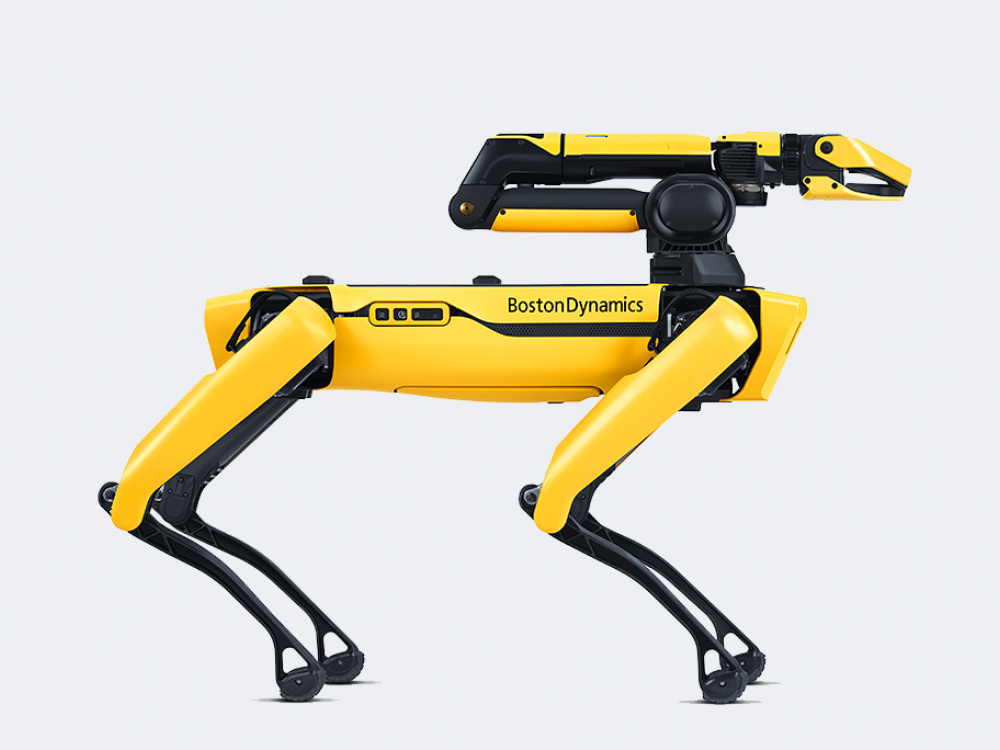
\includegraphics[width=0.5\textwidth]{figures/spot-arm-new-gray2x.png}
    \caption{Spot\textsuperscript{\textregistered} (credit to Boston Dynamics)}
    \label{fig:Spot}
\end{figure}
We are aiming on developing a free open source library of algorithms to mimic the behaviors of Spot\textsuperscript{\textregistered}.
In this project I worked on developing quadratic program inverse dynamics for Spot\textsuperscript{\textregistered} 
with an Arm as one small step towards our target. I used Drake\textsuperscript{\textregistered} library to implement this project.
This report is organized as follows:
\begin{itemize}
    \item Building the Model.
    \item PID Controller Implementation.
    \item Quadratic Program Implementation.
    \item Results.
    \item Future Work.
\end{itemize}

\section{Building the Model}
I downloaded the URDF files for the Spot\textsuperscript{\textregistered} and the arm from \url{https://github.com/heuristicus/spot_ros}
It was built for ROS.  It used stl file format for collision geometry while Drake\textsuperscript{\textregistered} accepts only Wavefront (obj) format.
It doesn't have inertial information. It doesn't have transmission (actuation) information.
I used Blender\textsuperscript{\textregistered} to convert stl files to Wavefront (obj) format.
I Used MeshLab\textsuperscript{\textregistered}  to get the inertial information from the obj files and the volume of the separate objects.
To calculate the mass of each object (torso, upper legs, and lower legs), I made a naive assumption as all these objects are made uniformly from the same material.
Based on the ration of the individual object volume to the total volume, I assigned mass to it so the total mass will match what Boston Dynamics has on their website.
And scaled the inertial tensor according to the newly assigned mass for each object. I added the transmission information. And as a last touch, I added four feet frames. One for each foot.
\begin{figure}
    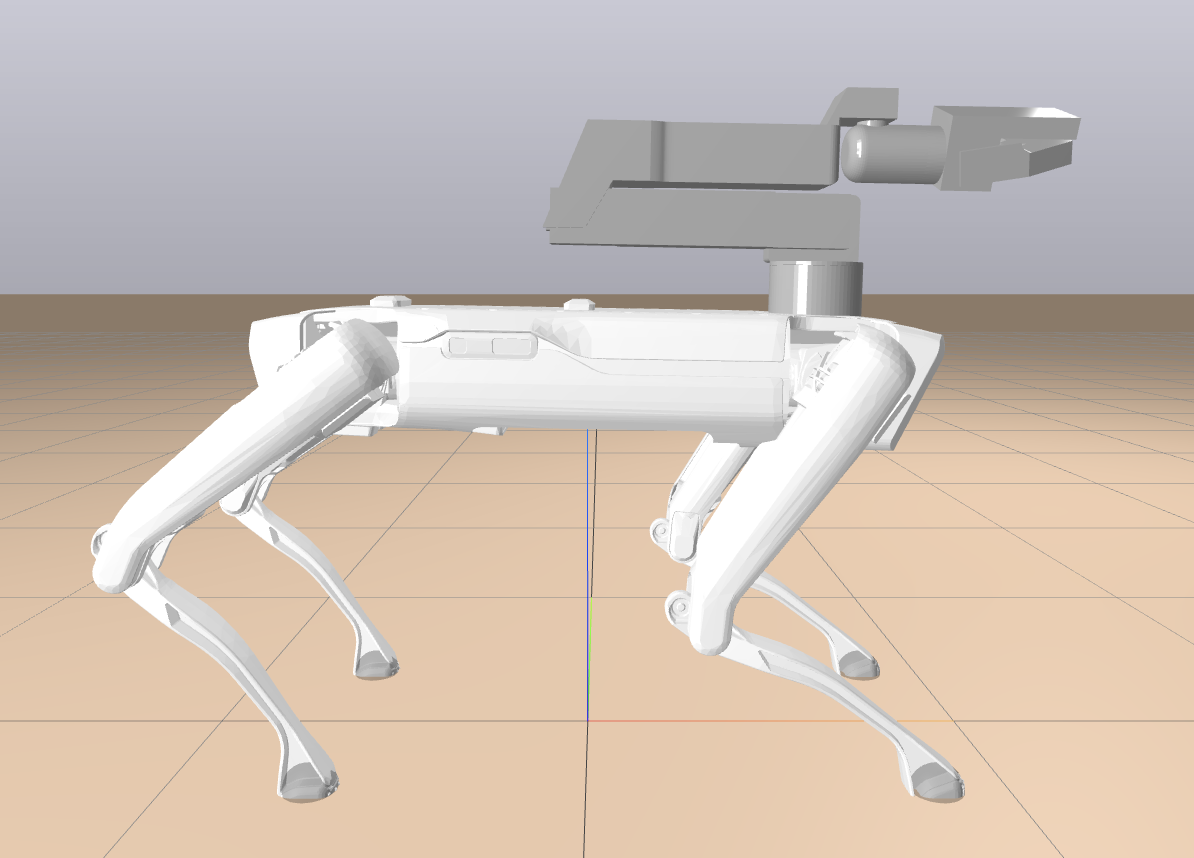
\includegraphics[width=0.5\textwidth]{figures/SpotModel.png}
    \caption{URDF model for Spot\textsuperscript{\textregistered}}
    \label{fig:SpotModel}
\end{figure}

\section{PID Controller Implementation}
The PID controller is a necessary subsystem to drive the robot to the desired state and stabilize it at that state. 
Yet it is not good to control the robot's center of mass projection on the ground by actuating the joints. 
Therefor we need the quadratic program in the next section. 
The main work I did is to extract the projection matrix to map the output estimated states vector $[q, v]$ from the plant to the desires 
state input of the PID controller. I used the LittleDog example we studied in class and modified it.
\begin{figure}
    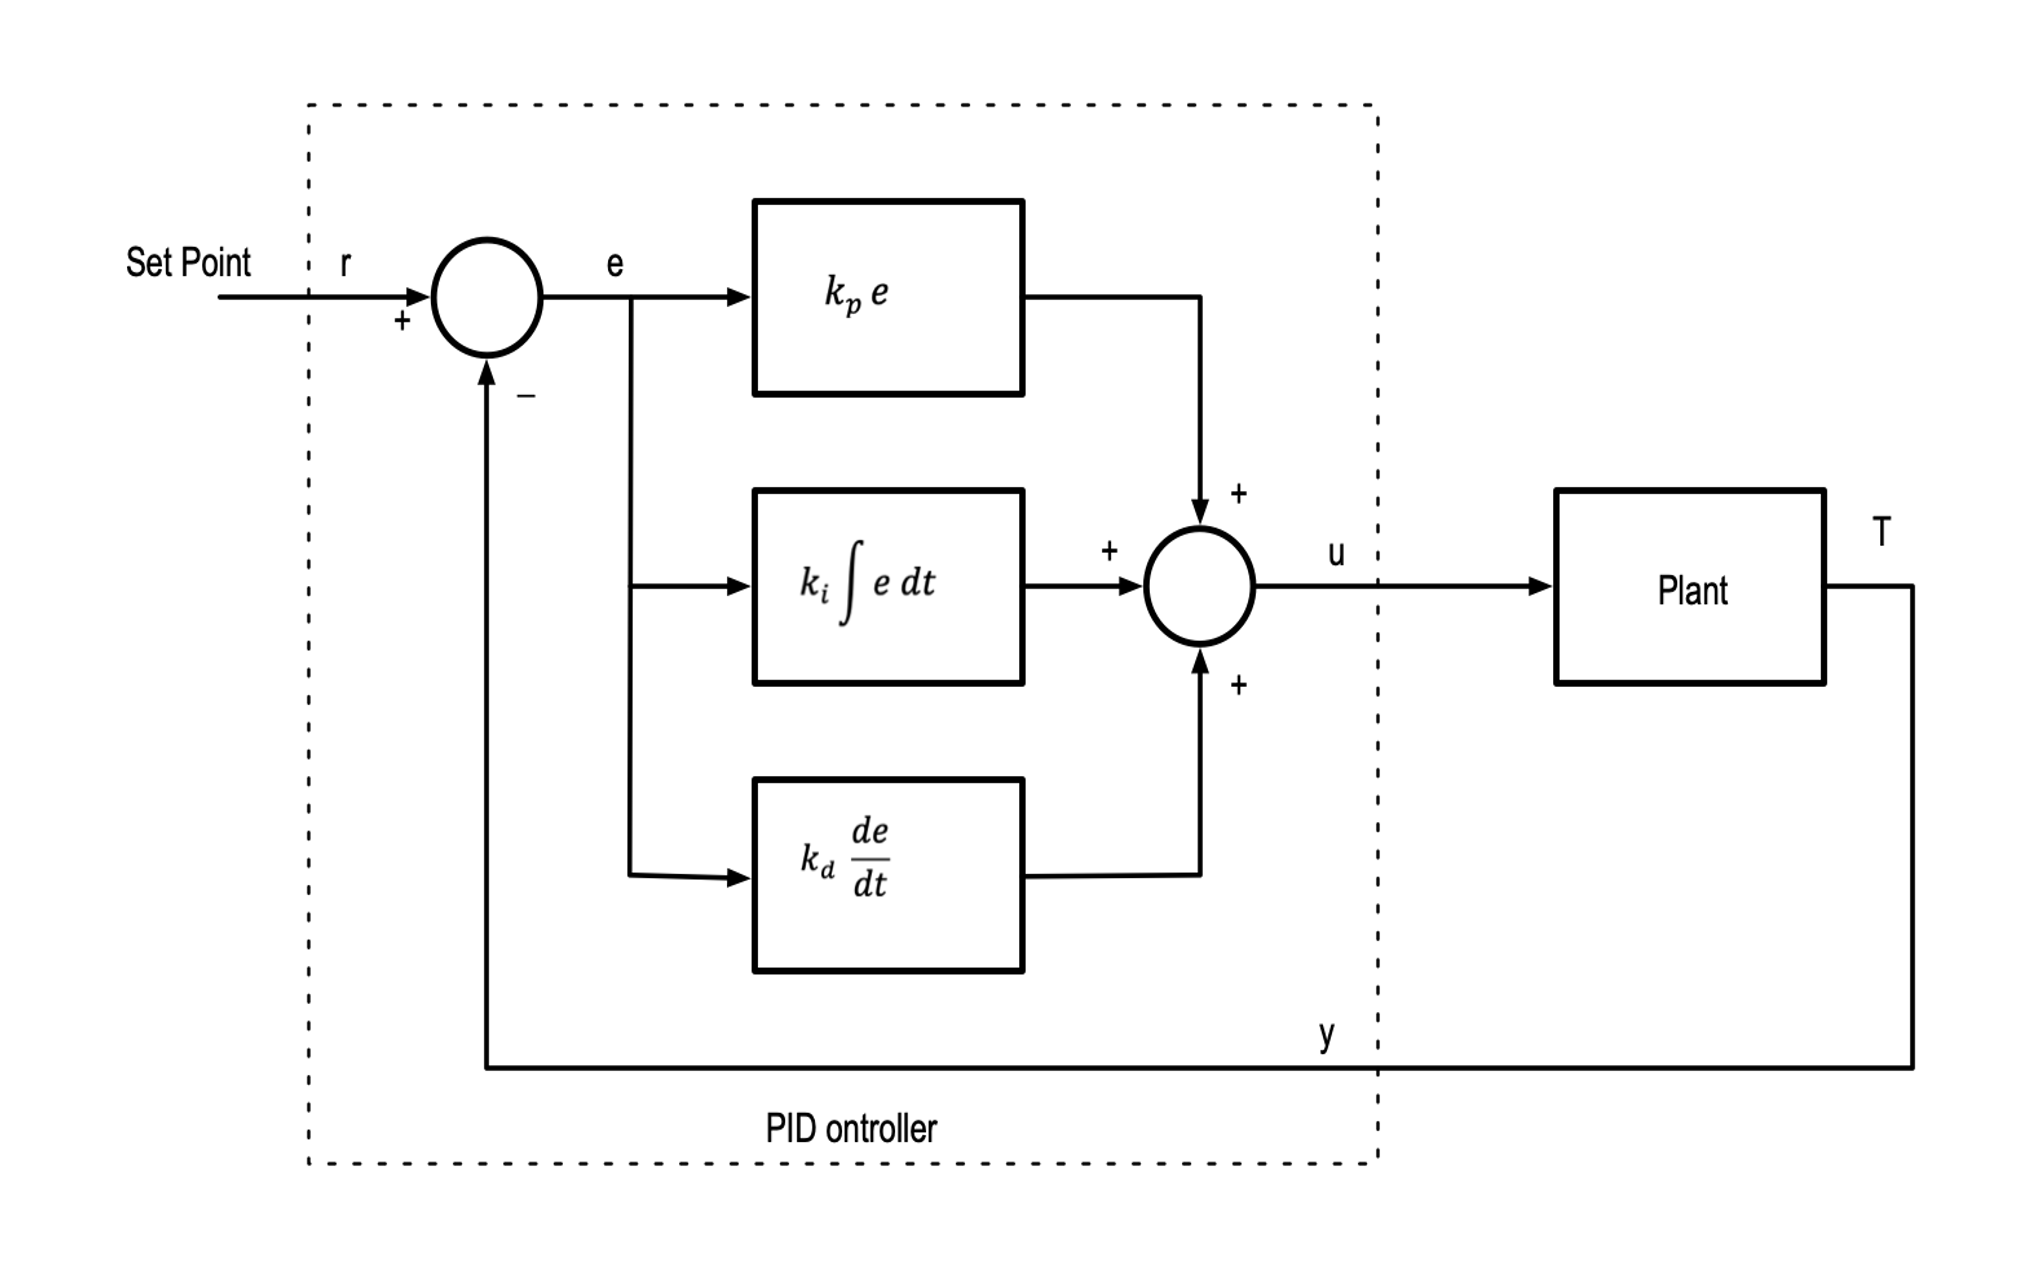
\includegraphics[width=0.5\textwidth]{figures/PID.png}
    \caption{PID Controller}
    \label{fig:PidController}
\end{figure}
I spent time on tuning the gains. For me it didn't stabilize with gains $K_p$ less than 100. I am currently using
$$K_p = 300$$
$$K_i = 3$$
$$K_d = 30$$

\section{Quadratic Program Implementation}
Givin $q$ and $v$ we can write the equations of motion
\begin{equation}
    H(q)\dot{v} + C(q,v) = B\tau + J^T\lambda
\end{equation}
\begin{equation}
    \begin{bmatrix}
        H_f\\
        H_a
    \end{bmatrix}\dot{v} + 
    \begin{bmatrix}
        C_f\\
        C_a
    \end{bmatrix}= 
    \begin{bmatrix}
        0\\
        B_a
    \end{bmatrix}\tau + 
    \begin{bmatrix}
        J_f^T\\
        J_a^T
    \end{bmatrix}\lambda
\end{equation}
The quadratic program formulation as in \cite{paper} is to: 
\begin{equation}
    \underset{q,v,\dot{v},\lambda}{minimize} l(
        \begin{bmatrix}
            q-q_{des}\\
            v-v_{des}
        \end{bmatrix}
        Q
        \begin{bmatrix}
            q-q_{des}\\
            v-v_{des}
        \end{bmatrix}^T
    )
\end{equation}
subject to:

\begin{equation} \tag{unactuated dynamics}
    H_f\dot{v} + C_f - J_f^T\lambda - \tau_g = 0
\end{equation}
\begin{equation} \tag{friction}
    \forall_{j=\{1..N_c\}}\lambda_f = \sum\limits_{i=1}^{N_d}\beta_{ij}w_{ij}
\end{equation}
\begin{equation} \tag{CoM inside the feet pressure cone}
    Ax_{CoM} - b \le 0
\end{equation}
\begin{figure}
    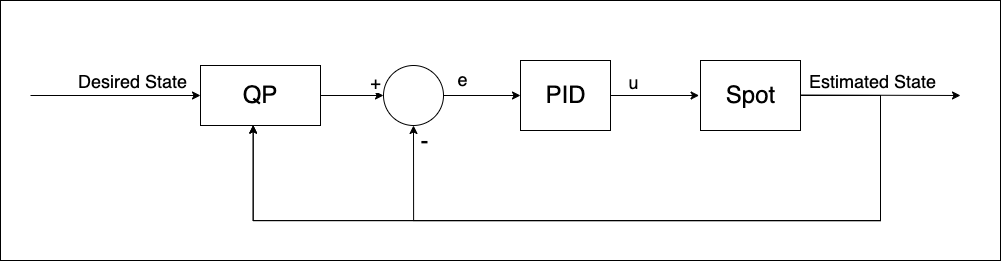
\includegraphics[width=0.5\textwidth]{figures/QP.png}
    \caption{Quadratic Program block diagram}
    \label{fig:QP}
\end{figure}
This problem is convex. SNOPT should be a good solver for convex quadratic program. 
Fig.4 shows the full system block diagram. The quadratic program will attempt to minimize the cost 
while respecting the constraints imposed on it.
according to my observation, it is very sensitive to the cost matrix $Q$. 

\section{Results}
When I reduced the hip roll cost on all the hips. It start behaving as I wanted.
\begin{figure}
    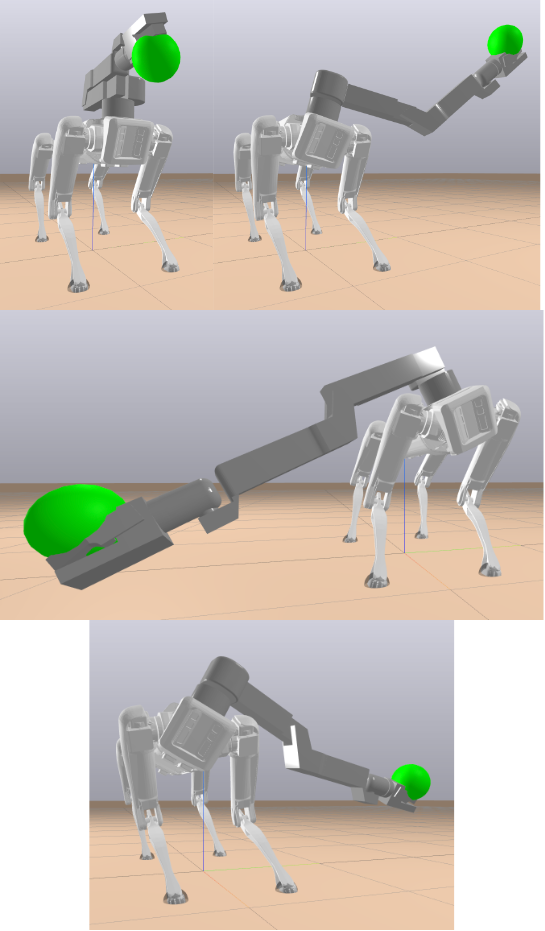
\includegraphics[width=0.5\textwidth]{figures/result.png}
    \caption{Result}
    \label{fig:result}
\end{figure}
\section{Discussion}
I made it work few hours before the due time. I am still testing it and trying to find issues and fix them.
The PID gains need to come down to manage to get the model sampling rate lower and that might speeds up the Optimization
and speeds up the testing.
I found out that SNOPT sometimes would violate some constraints and still report success for the solution.
During my testing sometimes before the optimizer crashes, I can see the location of the feet frames and the center of mass changes
while the robot is not moving. I think there are some plant-context and sim-context mix up. I need to dig into this issue.

\section{Future Work}
More fine tuning and some adjustments are needed for this project to make it reliable and robust. The structure of the code 
makes the QP solver very slow. It worth putting time on making it run faster.
Besides improving this project. This project is just the start of many more projects to build the open source library.

\begin{thebibliography}{}
    \bibitem{paper}
    Scott Kuindersma, Robin Deits, Maurice Fallon, Andr\'{e}s Valenzuela, Hongkai Dai, 
    Frank Permenter, Twan Koolen, Pat Marion, Russ Tedrake 
    \emph{Optimization-based Locomotion Planning, Estimation, and Control Design for the Atlas Humanoid Robot}
\end{thebibliography}
\end{document}
